\documentclass[../../main.tex]{subfiles}  % Same level as chapter file, so same path
\graphicspath{{\subfix{../Plots/}}}

\begin{document}

\section{Examples}

	\subsection{Citations, figures, tables}

	Hooray for Chapter 2!!! Here's an example of citing things, I'm going to cite a brilliant paper - \supercite{aartsSolutionDependencyUsing2014}. See bibliography.bib for doing references.

	\begin{figure*}
		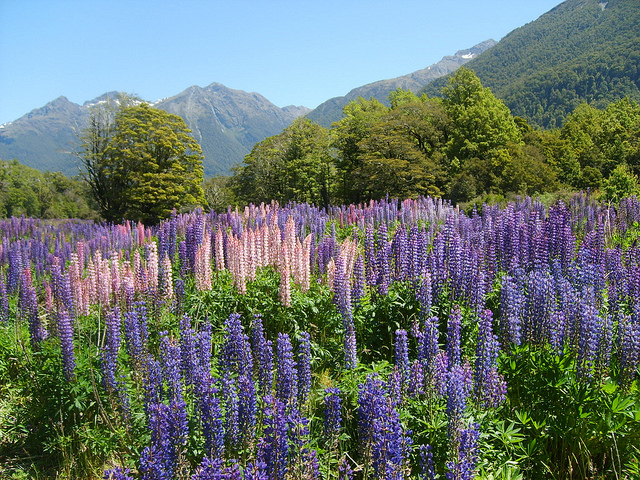
\includegraphics[height =5in]{./Plots/nature.jpg}
		\caption{An individual figure!}
	\end{figure*}
			
	\begin{figure*}[h]
		\subfloat[\label{fig:HD8538_ellplot}]{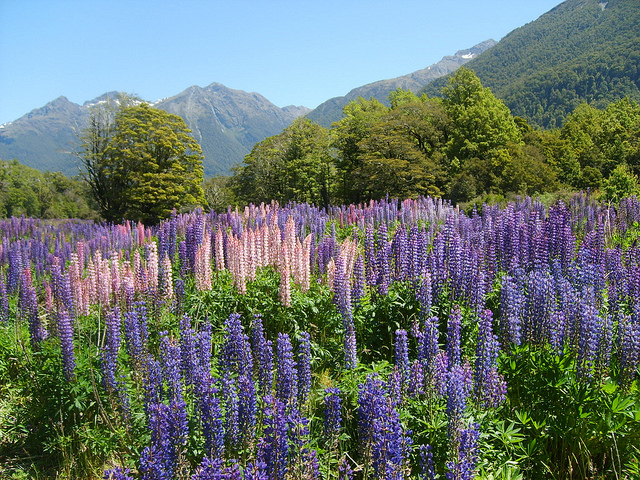
\includegraphics[height =2.5in]{./Plots/nature.jpg}} 
		\subfloat[\label{fig:HD8538_phot}]{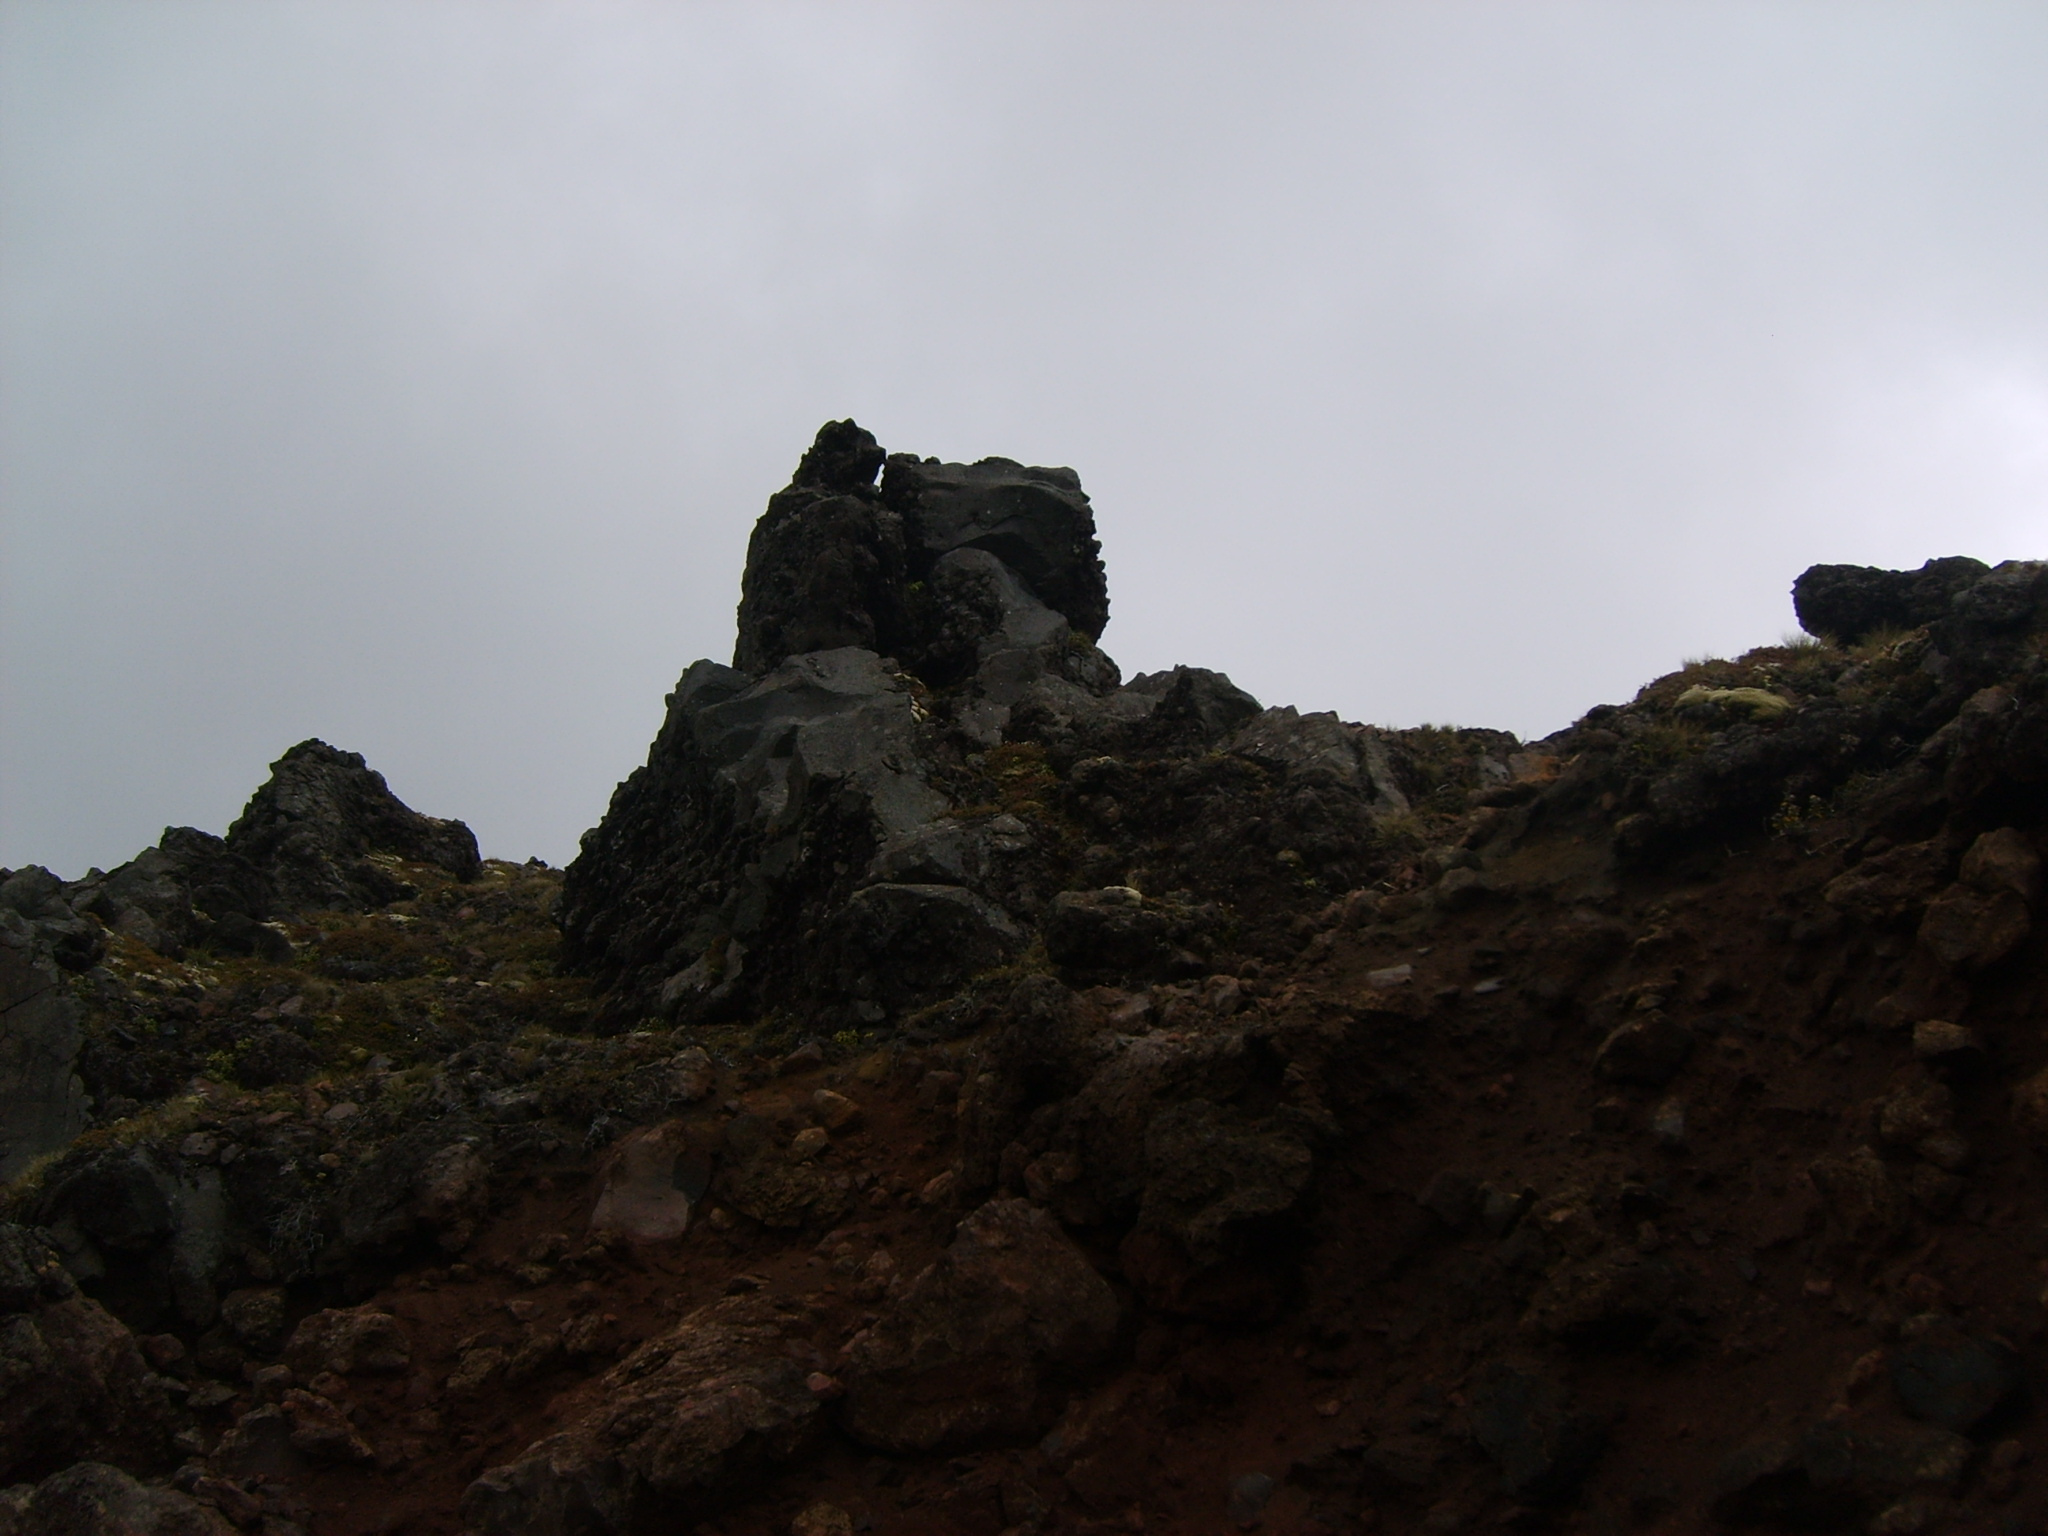
\includegraphics[height =2.5in]{./Plots/rocks.jpg}} \\
		\subfloat[\label{fig:HD8538_vis}]{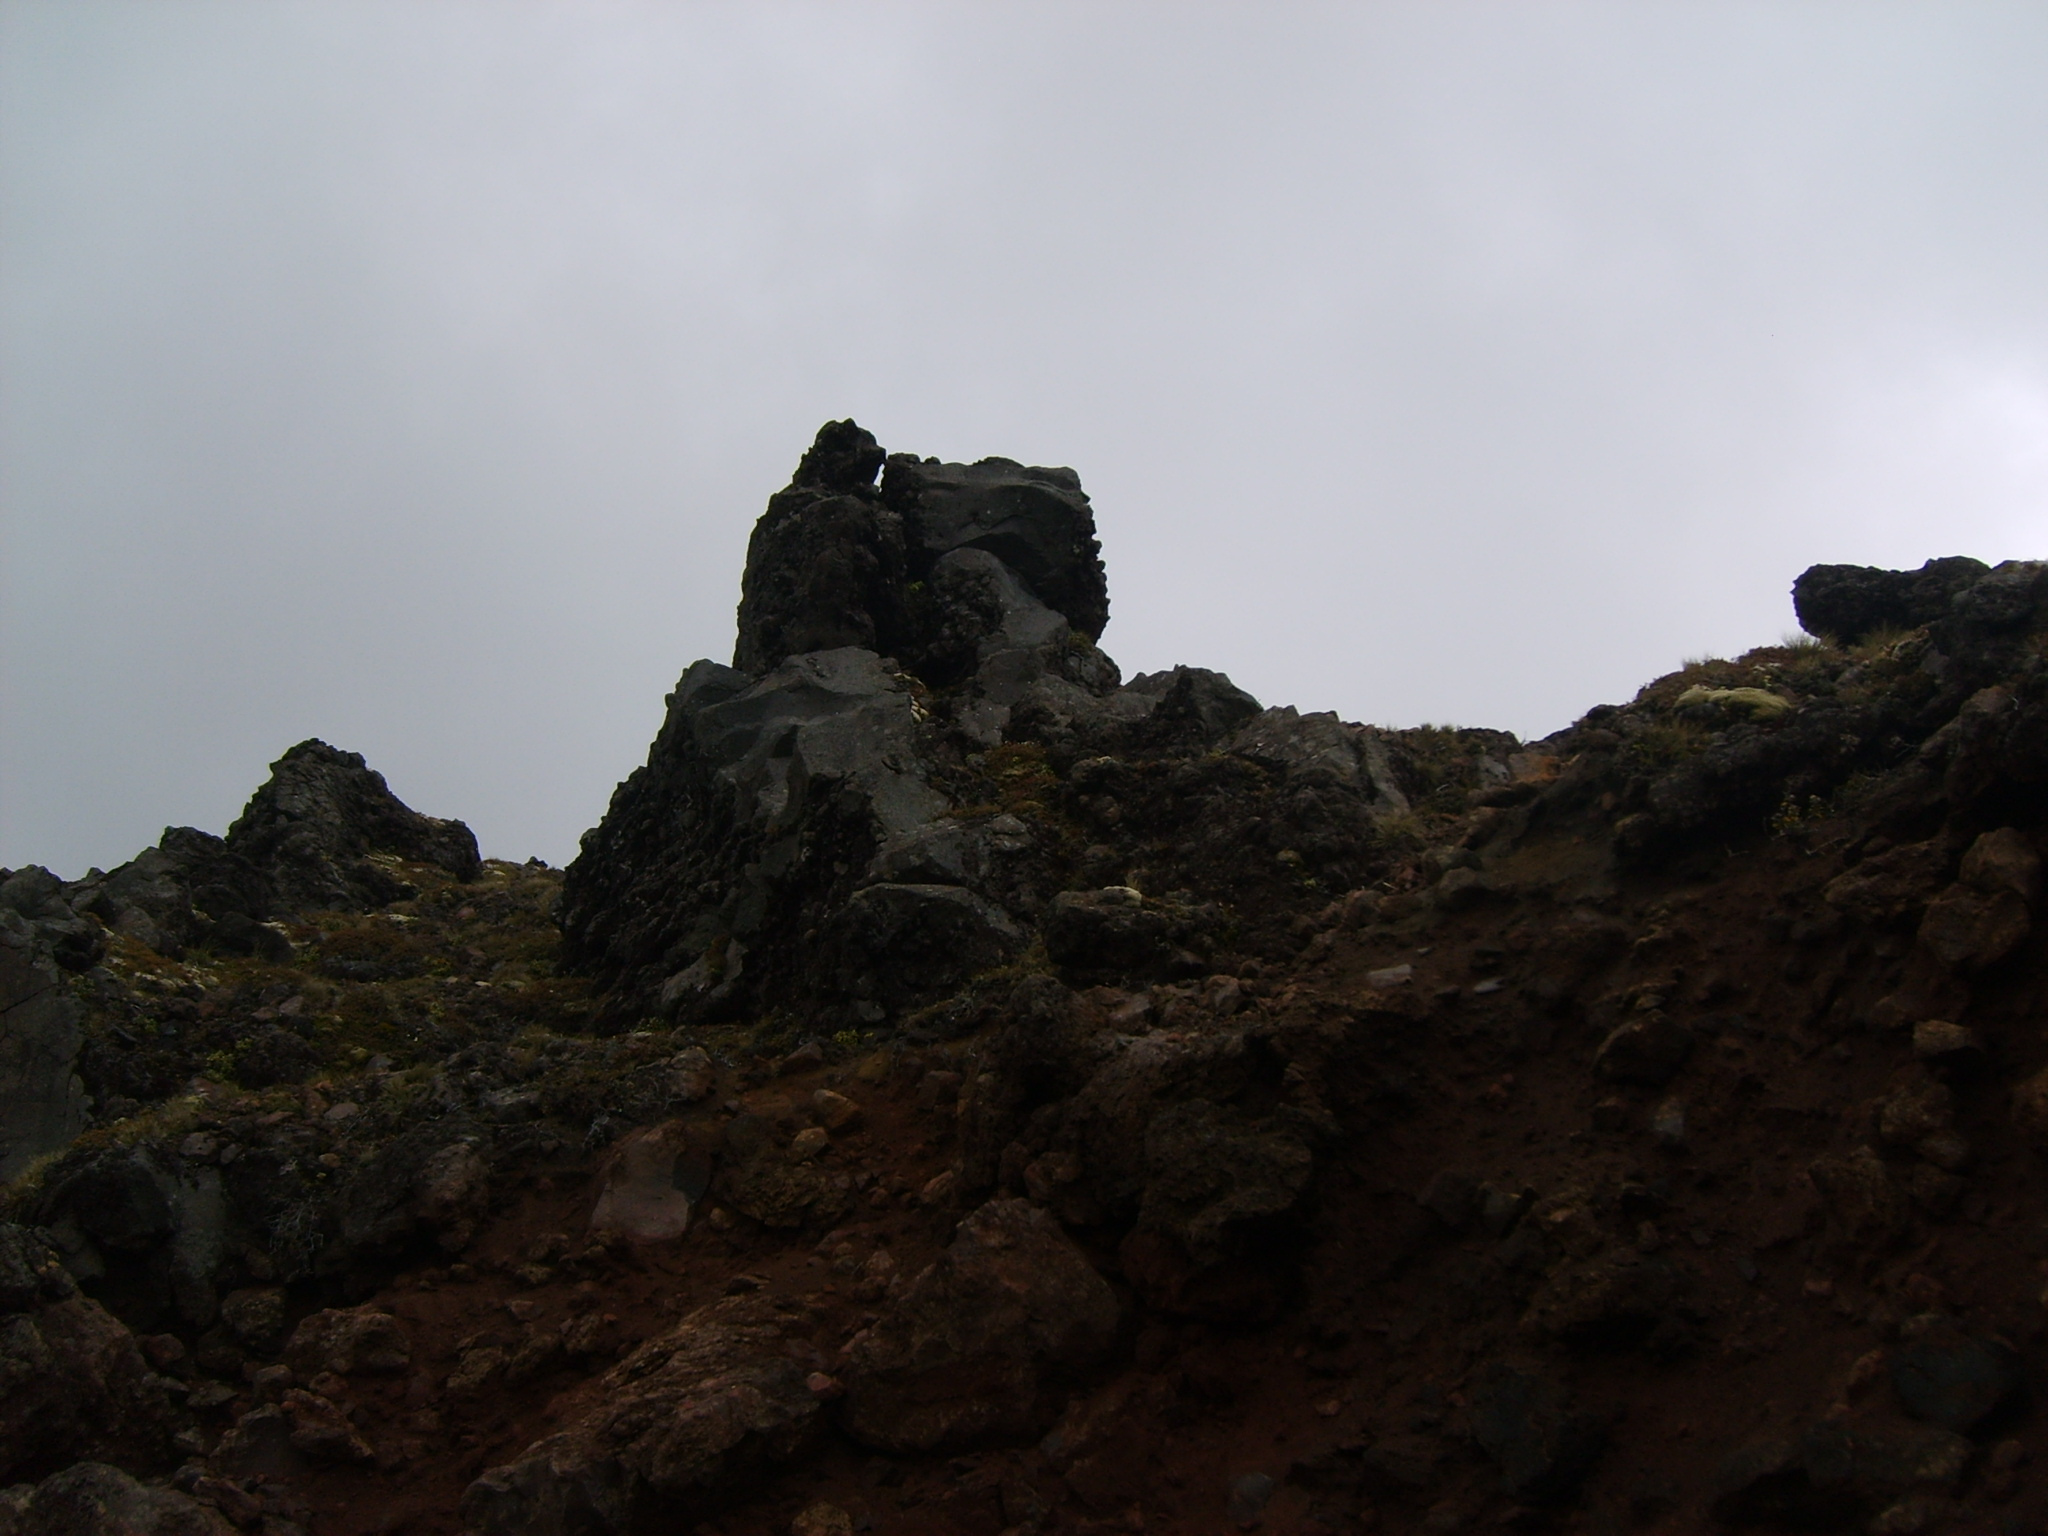
\includegraphics[height =2.5in]{./Plots/rocks.jpg}}
		\subfloat[\label{fig:HD8538_HRD}]{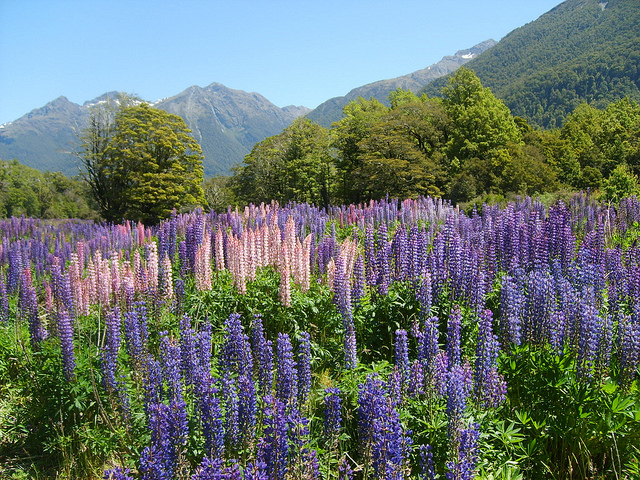
\includegraphics[height =2.5in]{./Plots/nature.jpg}}
		\caption{Multiple figures!}
	\end{figure*}


	\begin{landscape}
\begin{longtable}{cccccccccccccc}
\label{tab:disk}\\
\caption{Insert Table Caption here}\\
\hline\endhead  % header material
\hline\endfoot  % footer material
\hline
Blah & Blah & Blah \\
\hline
Stuff & Things & etc. \\
\nodata & \nodata & \nodata \\
\end{longtable}
\end{landscape}

	\subsection{Abbreviations and SI units}

	Here are some examples of more complex use-cases for abbreviations and SI units. 

\end{document}